% !TEX root = main.tex

\section{非参数技术} % 4.1-4.6
\subsection{概率密度的估计}
向量$\vx$落在区域$\mR$的概率为
\[P=\int_{\mR}p(\vx')\diff\vx'\]
即$P$是概率密度函数$p(\vx)$平滑后的版本。
若假设$p(\vx)$是连续的,且区域$\mR$足够小,以致于在这个区间中$p$几乎没有变化,则
\[\int_{\mR}p(\vx')\diff\vx'\approx p(\vx) V\]
其中$\vx$为一个点,而$V$为区域$\mR$所包含的体积。
可以用下述公式作为一个估计
\[p(\vx)\approx\frac{k/n}{V}\]
即从$n$个服从$p(\vx)$的独立同分布样本落在$\mR$中的有$k$个。

为了估计$\vx$的概率密度函数,构造一系列包含$\vx$的区域$\mR_1,\mR_2,\ldots$,第一个区域用$1$个样本,第二个区域用$2$个,以此类推。
$V_n$为区域$\mR_n$的体积,$k_n$为落在区间$\mR_n$中的样本个数,而$p_n(\vx)$表示对$p(\vx)$的第$n$次估计:
\[p_n(\vx)=\frac{k_n/n}{V_n}\]
若要求$p_n(\vx)$能够收敛到$p(\vx)$,则下面3个条件必须满足:
\begin{itemize}
	\item $\lim_{n\to\infty}V_n=0$
	\item $\lim_{n\to\infty}k_n=\infty$
	\item $\lim_{n\to\infty}k_n/n=0$
\end{itemize}
第一个条件保证区域均匀收缩和$p(\cdot)$在点$\vx$除连续的情况下,区间平滑了的$P/V$能够收敛到$p(\vx)$。
第二个条件保证频率之比能够收敛到概率$P$。
最后一个条件说明虽然最后落在小区域$\mR_n$中的样本数目非常大,但是这么多样本在全体样本中所占的比例非常小。

\subsection{Parzen窗方法}
假设区间$\mR_n$是$d$维超立方体,$h_n$为一条边长度,体积为
\[V_n=h_n^d\]
定义窗函数
\[\varphi(\vu)=\begin{cases}
1 & |\vu_j|\leq 1/2,\;j=1,\ldots,d\\
0 & \text{其他}
\end{cases}\]
这样$\varphi(\vu)$就表示一个中心在原点的单位超立方体。
若$\vx_i$落在中心点为$\vx$的立方体$V_n$中,那么
\[\varphi((\vx-\vx_i)/h_n)=1\]
否则为$0$,进而可解析表达超立方体样本个数
\[k_n=\sum_{i=1}^n\varphi\lrp{\frac{\vx-\vx_i}{h_n}}\]
代入估计式有
\[p_n(\vx)=\frac{1}{n}\sum_{i=1}^n\frac{1}{V_n}\varphi\lrp{\frac{\vx-\vx_i}{h_n}}\]

\subsection{$k_n$近邻估计}
最佳的窗函数的选择是个问题,因此一种可行的方案是让体积成为训练样本的函数,而不是硬性规定窗函数为样本个数的某个函数。

比如说可以取$k_n=\sqrt{n}$,有下列迭代过程。
\begin{figure}[H]
\centering
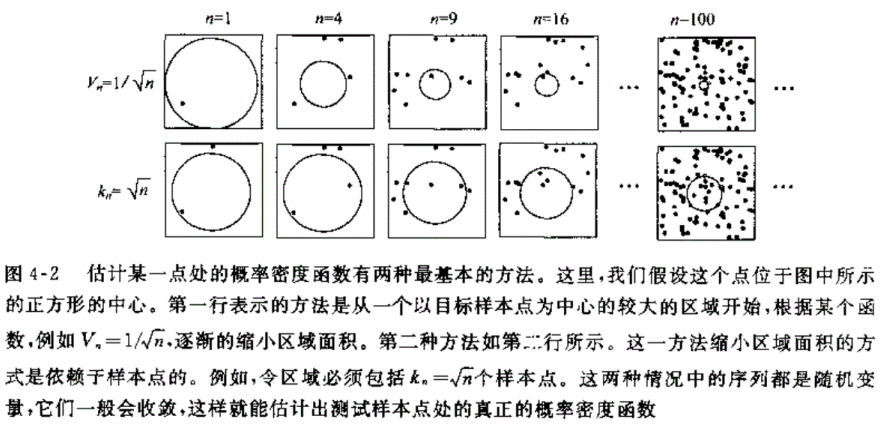
\includegraphics[width=0.8\linewidth]{fig/kn-neighbor.png}
\end{figure}

\subsection{最近邻规则}
定义$\omega_m(\vx)$为
\[P(\omega_m\mid\vx)=\max_i P(\omega_i\mid\vx)\]
记$n$个样本的平均误差率为$P_n(e)$,且
\[P=\lim_{n\to\infty}P_n(e)\]
则希望证明
\[P^*\leq P\leq P^*\lrp{2-\frac{c}{c-1}P^*}\]

进而推广有$k$近邻规则(KNN)。